\documentclass[10pt,a4paper]{report}
\usepackage[utf8]{inputenc}
\usepackage[spanish]{babel}
\usepackage{amsmath}
\usepackage{amsfonts}
\usepackage{amssymb}
\usepackage{lmodern}
\usepackage[left=2cm,right=2cm,top=2cm,bottom=2cm]{geometry}
\usepackage{makeidx}
\usepackage{graphicx}
\usepackage{lmodern}


\title{Resumen Paradigmas de la Programación\\~\\Licenciatura en Ciencias de la 
Computación\\FaMAF-UNC}
\author{Agustin Curto     agucurto95@gmail.com}
\date{2016}

\begin{document}
\tableofcontents

\chapter{Qué es y qué puede hacer un lenguaje de programación}

Un lenguaje de programación es un lenguaje formal disenñado para realizar 
procesos que pueden ser llevados a cabo por máquinas como las 
computadoras. Pueden usarse para crear programas que controlen el 
comportamiento físico y lógico de una máquina o para expresar algoritmos 
con precisión.

\section{Sintáxis y Semántica}

\par Los lenguajes son sistemas que se sirven de una forma para comunicar 
un significado. Lo que tiene que ver con la forma recibe el nombre de 
sintaxis y lo que tiene que ver con el significado recibe el nombre de semántica.

\par En los lenguajes de programación, que son lenguajes artificiales 
creados por hombres (lenguajes formales), la forma son los programas y el 
significado es lo que los prográmas hacen, usualmente, en una 
computadora. En la definición de arriba, se ha descrito lo que los programas 
como “controlar el comportamiento físico y lógico de una máquina”.
Un lenguaje de programación se describe con su sintaxis (qué es lo que se 
puede escribir legalmente en ese lenguaje) y su semántica (qué efectos 
tiene en la máquina lo que se escribe en ese lenguaje).

\par La implementación de un lenguaje de programación debe transformar 
la sintáxis de un programa en instrucciones de máquina que se pueden 
ejecutar para que suceda la secuencia de acciones que se pretendía.
El compilador hace esa traducción, un intérprete puede combinar traducción 
y ejecución.


\section{ Sintáxis a traves de gramáticas}

\par Vamos a estar usando gramáticas independientes de contexto, más 
específicamente EBNF, que es el estándar de facto para estas gramáticas; 
aunque algunas propiedades de los lenguajes de programación escapan a su 
expresividad.

\par Un gramática es un método para definir conjuntos infinitos de 
expresiones y procesar expresiones. Consisten de: 

	\begin{itemize}
		\item símbolo inicial
		\item no terminales
		\item terminales
		\item producciones
	\end{itemize}

\par Los no terminales son la forma adecuada de describir la 
composicionalidad de las expresiones, no pueden formar parte de una 
expresión, siempre se tienen que substituir por terminales.


\chapter{Cómo funcionan los lenguajes de programación}

\section{Compilador}
\par El compilador es un programa que lee un programa escrito en un 
lenguaje origen y lo traduce a un programa equivalente en un lenguaje destino, 
normalmente el lenguaje origen es de alto nivel y el destino es de bajo nivel. El 
mismo posee dos componentes:

	\begin{itemize}
		\item Entender el programa (asegurarse de que es correcto)
		\item Reescribir el programa
	\end{itemize}

\subsection{Fases de un compilador}

\begin{enumerate}
	\item \underline{Análisis léxico:} se divide un programa (secuencia de caracteres) en 
	palabras (tokens).
	
	\item \underline{Análisis sintáctico:} comprueba si la secuencia de tokens conforma 
	a la especificación gramatical del lenguaje y genera el árbol sintáctico. La 
	especificación gramatical suele representarse con una gramática 
	independiente de contexto, que también le da forma al árbol sintáctico.
	
	\item \underline{Análisis semántico:} El compilador trata de ver si un un programa 
	tiene sentido analizando su árbol sintáctico. Un programa sin errores 
	gramaticales no siempre es correcto, puede haber problemas de tipo:

  	\begin{equation}
  		pos =  init + rate * 60
  	\end{equation}
	
		\par Qué pasa si pos es una clase y init y rate son enteros. El parser 
		no puede encontrar este tipo de errores, el análisis semántico 
		encuentra este tipo de error.

		\par El compilador hace comprobaciones semánticas estáticas (static 
		semantic checks): 
		\begin{itemize}
			\item comprobación de tipos
			\item declaración de variables antes de su uso
			\item se usan los identificadores en contextos adecuados 
			\item comprobar argumentos
		\end{itemize}

		\par Si hay un fallo en compilación, se genera un error en tiempo de 
		ejecución (dynamic semantic checks) se comprueba:
		\begin{itemize}
		\item que los valores de los arreglos estén dentro de los límites
		\item errores aritméticos (división por 0)
		\item no se desreferencian los punteros si no apuntan a un objeto 
		válido 
		\item se usan variables sin inicialización
		\item si hay un fallo en ejecución, se levanta una excepción
		\end{itemize}
		
		\subsubsection{Tipado fuerte}
			
		\par Un lenguaje tiene tipado fuerte si siempre se detectan los errores 
		de tipo:
		\begin{itemize}
			\item En tiempo de compilación o de ejecución
			\item Tipado fuerte: Ada, Java, ML, Haskell
			\item Tipado débil: Fortran, Pascal, C/C++, Lisp 
			\item Duck typing: Python
		
		\par El tipado fuerte hace que el lenguaje sea más seguro y fácil de 
		usar sin errores, pero potencialmente más lento por las 
		comprobaciones dinámicas. En algunos lenguajes algunos errores de 
		tipo se detectan tarde, lo que los hace poco fiables (Basic, Lisp, 
		Prolog, lenguajes de scripting).
		\end{itemize}
		
	\item \underline{Generación y optimización de código intermedio:} El código 
	intermedio está cerca de la máquina pero sigue siendo fácil de manipular, 
	para poder implementar optimizaciones. Por ejemplo:
	
	\begin{equation}
	 temp1 = 60
	 \end{equation}
	 \begin{equation}
     temp2 = id3 + temp1
     \end{equation}
     \begin{equation}
     temp3 = id2 + temp2
     \end{equation}
     \begin{equation}
     id1 = temp3 
     \end{equation}

	\par Se puede optimizar (independientemente de máquina):
     \begin{equation}
     temp1 = id3 * 60.0
     \end{equation}
     \begin{equation}
     id1 = id2 + temp1 
		\end{equation}

	\item \underline{Generación y optimización de código destino:} De la forma 
	independiente de máquina se genera ensamblador:
	\begin{equation}
	 MOVF id3, R2
	 \end{equation}
	 \begin{equation}
     MULF 60.0, R2
     \end{equation}
     \begin{equation}
     MOVF id2, R1
     \end{equation}
     \begin{equation}
     ADDF R2, R1
     \end{equation}
     \begin{equation}
  	 MOVF R1, id1
     \end{equation}
     
     \par Este código específico de máquina se optimiza para explotar 
     características de hardware específicas.
	
\end{enumerate}


\section{Paradigma Imperativo}

\par Un paradigma de programacón es una configuracón frecuente de 
características de lenguajes de programacón. El paradigma imperativo es el 
más antiguo y el que estuvo siempre más pegado a la máquina. 
Tradicionalmente se ha opuesto al paradigma funcional, pero la mayor parte 
de lenguajes integran ideas de ambos paradigmas.

\subsection{Conceptos fundamentales}

	\begin{itemize}
	 	\item Operación básica: \textbf{asignación}. La asignación tiene 
	 	efectos secundarios ya que cambia el estado de la máquina.
		\item Sentencias de \textbf{control} de flujo: condicionales y sin 
		condición (GO TO), ramas, ciclos.
		\item Bloques, para obtener \textbf{referencias locales}
  		\item \textbf{Parametrización}
	\end{itemize}

\subsection{Elementos básicos}
  	
  	\begin{enumerate}
		\item Definiciones de \textbf{tipos}
		\item Declaraciones de \textbf{variables} (normalmente tipadas)		
 		\item Expresiones y sentencias de \textbf{asignación}
 		\item Sentencias de \textbf{control de flujo} (normalmente 
		estructuradas)
 		\item \textbf{Alcance léxico} y bloques, para poder tener variables 
 		con referencias locales
		\item Declaraciones y definiciones de \textbf{procedimientos} y 
		\textbf{funciones} (bloques parametrizados)
	\end{enumerate}
		
\subsection{Declaraciónes de variables}
		\par Las declaraciones tipadas restringen los posibles valores de una 
		variable en la ejecución del programa:
		\begin{itemize}
		\item Jerarquía de tipos built-in o personalizada
		\item inicialización
		\end{itemize}
		
		\par Uso de memoria: cuánto espacio de memoria reservar para cada
		tipo de variable.
		
\subsection{Ubicación y valores de variables}
		\par Al declarar una variable la estamos ligando a una 
		\textbf{ubicación en memoria}, de forma que el nombre de la variable 
		es el identificador de la ubicación en memoria. La ubicación puede ser 
		global, en la pila o en el heap.
		
		\begin{itemize}
		\item l-valor: ubicación en memoria (dirección de memoria)
		\item r-valor: valor que se guarda en la ubicación de memoria 
		identificada por el l-valor
		\end{itemize}
		
		\par La asignación: A (objetivo) = B (expresión), es una actualización 
		destructiva, ya que reescribe la ubicación de memoria identificada por 
		A con el valor de la expresión B.

\subsection{Semántica de copia vs. Semántica de referencia}
		\begin{itemize}
		\item Semántica de copia: la expresión se evalúa a un valor, que se 
		copia al objetivo (lenguajes imperativos).
		\item Semántica de referencia: la expresión se evalúa a un objeto, 	
		cuyo puntero se copia al objetivo (lenguajes orientados a objetos).
		\end{itemize}

\subsection{Variables y asignación}
		\par En la parte derecha de una asignación está el r-valor de la 
		variable, en la parte izquierda está su l-valor. Una expresión que no 
		tenga un l-valor no puede aparecer en la parte izquierda de una 
		asignación. El r-valor de un puntero es el l-valor de otra variable (el 
		valor de un puntero es una dirección).
		
		\begin{itemize}
		\item las constantes sólo tienen r-valor
 		\item las funciones sólo tienen l-valor
		\end{itemize}

		\subsubsection{L-valor y R-valor en C}
		\begin{itemize}
		\item \&x devuelve el l-valor de x 
    	\item *p devuelve el r-valor de p. Si p es un puntero, esto es el l-valor 
    	de otra variable
		\end{itemize}

\subsection{Control de flujo estructurado}

\par Se piensa como secuencial, las instrucciones se ejecutan en el orden en el que están escritas, en algunos casos soporta ejecución concurrente. \par Un programa es estructurado si el flujo de control es evidente en la estructura sintáctica del texto del programa. Esto es 	útil para poder razonar intuitivamente leyendo el texto del programa, ya que se crean construcciones del lenguaje para patrones comunes de control: iteración, selección, procedimientos, funciones, etc.

		\subsubsection{Estilo moderno}
		\par Construcciones estándar que estructuran los saltos: 
		\begin{itemize}
			\item if ... then ... else ... end 
			\item while ... do ... end
			\item for ...{...}
			\item case ...
		\end{itemize}
		
		\par Se agrupa el código en bloques lógicos, se evitan saltos explícitos 
		(excepto retorno de función), no se puede saltar al medio de un 
		bloque o función.


\chapter{Estructura en bloques}

\section{Estructura de bloque}
\subsubsection{Manejo de memoria}
		\begin{itemize}
			\item Al stack tiene los datos sobre entrada y salida de bloques
			\item El heap tiene datos de diferente lifetime
			\item El puntero de entorno (environment) apunta a la posición 
			actual en el stack
			\item Al entrar a un bloque: se añade un nuevo activation record al 
			stack
			\item Al salir de un bloque: se elimina el activation record más 
			reciente del stack
		\end{itemize}
		
\subsection{Alcance y lifetime}
\begin{itemize}
\item Alcance: región del texto del programa donde una declaración es 
visible.
\item Lifetime: período de tiempo en que una ubicación de memoria es asignada a un programa.
\end{itemize}

\section{Activation records}

\par Para describir la semántica de los lenguajes de programación, más 
específicamente lenguajes estructurados por bloques, usamos una 
semántica operacional, es decir, describimos los efectos de las diferentes 
expresiones del lenguaje sobre una máquina. Para eso usamos un modelo 
simplificado de la computadora, el que se ve en la figura.

\begin{center} 
	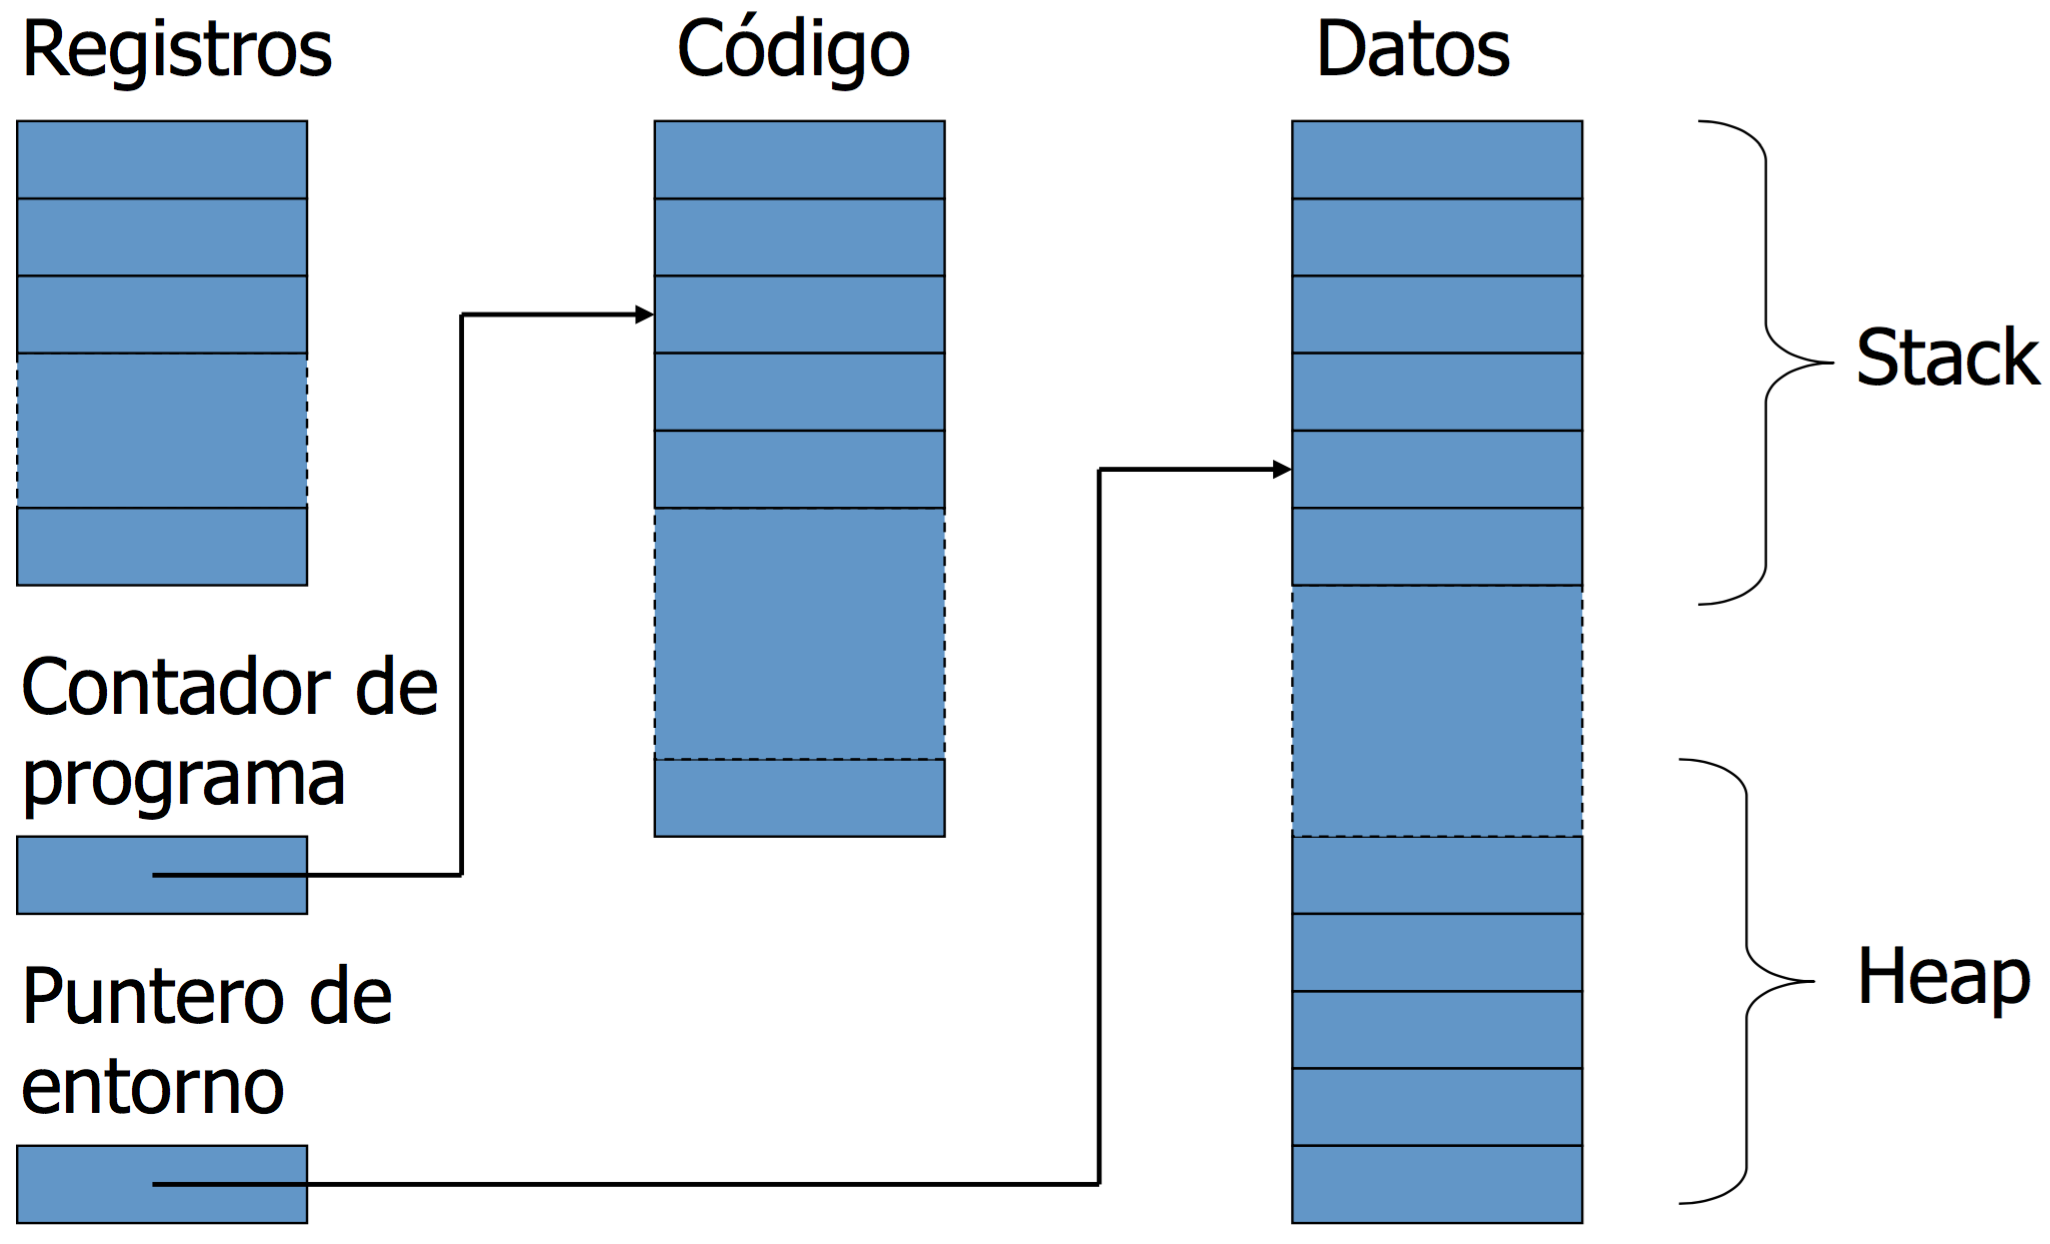
\includegraphics[width=12cm, height=6cm]{arecord.png}
\end{center}

\par Vemos que este modelo de máquina separa la memoria en la que se 
guarda el código (\textbf{stack}), de la memoria en la que se guardan los 
datos (\textbf{heap}). Usamos dos variables para saber a qué parte de la 
memoria necesitamos acceder en cada momento de la ejecución del 
programa: el \textbf{contador de programa}, que es una dirección en la 
parte de la memoria donde se guarda el código, en concreto, la dirección 
donde se encuentra la instrucción de programa que se está ejecuntando 
actualmente y y el \textbf{puntero de entorno}, el cual nos sirve para 
saber cuáles son los valores que se asignan a las variables que se están 
usando en una parte determinada del código. 

\par Cuando el programa entra en un nuevo bloque, el stack se encarga de agregar una estructura de datos que se llama \textbf{\textit{activation record}}, que contiene el espacio para las variables locales declaradas en el bloque, normalmente, por la parte de arriba de la pila. Entonces, el puntero de entorno apunta al nuevo activation record.

\par Cuando el programa sale del bloque, se retira el activation record de la pila y el puntero de entorno se restablece a su ubicación anterior, es decir, al puntero de entorno correspondiente a la función que llamaba a la función que ha sido desapilada. El activation record que se apila más recientemente es el primero en ser desapilado, a esto se le llama disciplina de pila.

\par Ademas el activation record posee espacio para guardar resultados intermedios, en el caso de que sea necesario. Podemos observar, en la figura siguiente, que hay dos direcciones de memoria donde se guardan datos importantes: el control link, contiene el que será el puntero de entorno cuando se desapile el activation record actual y la dirección de memoria distinguida es la llamada dirección de retorno, que es donde se va a guardar el resultado de la ejecución de la función, si es que lo hay.

\begin{center} 
		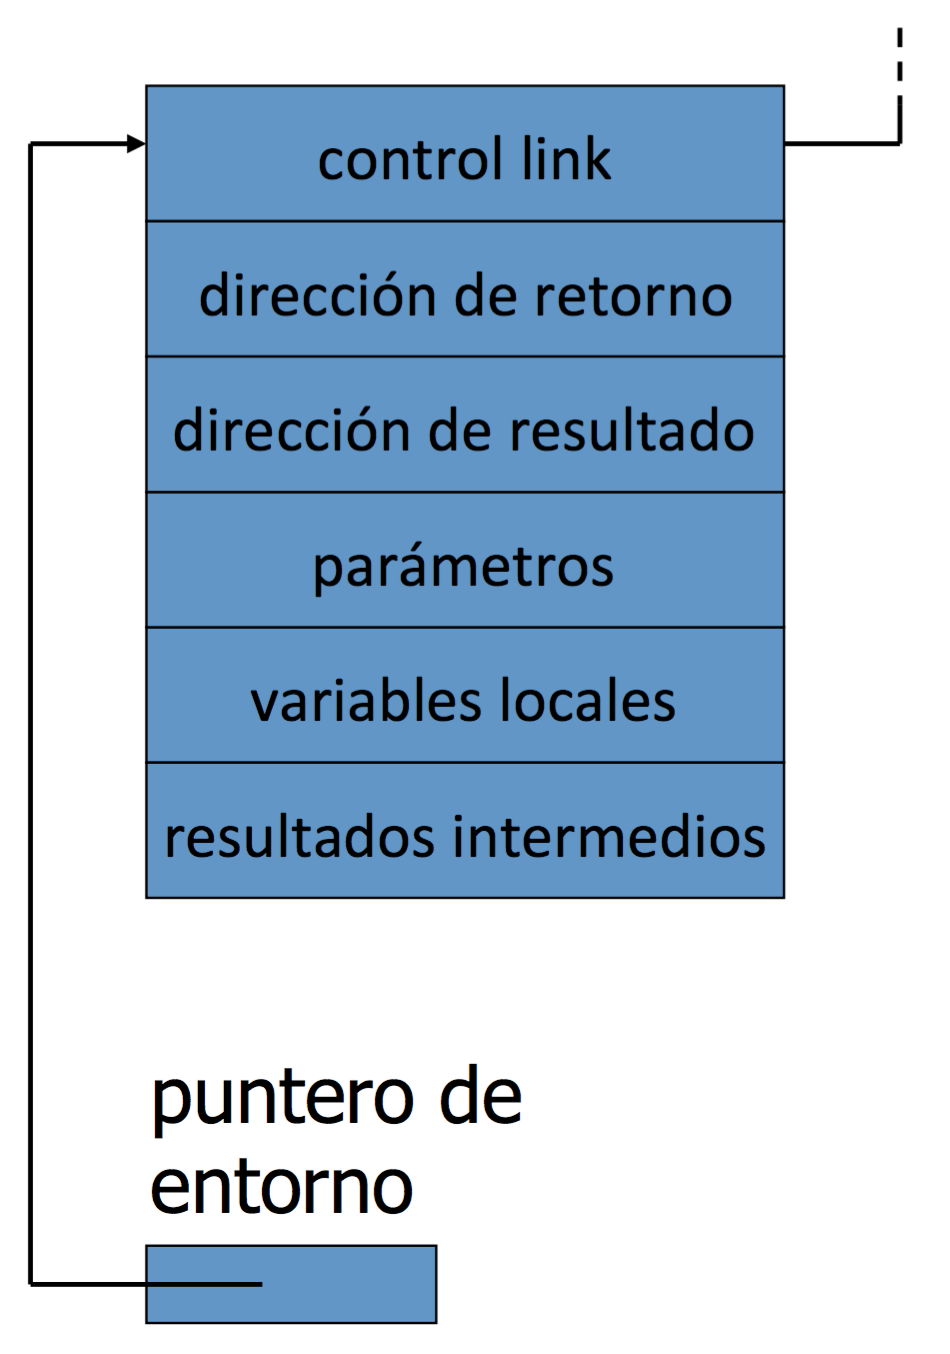
\includegraphics[width=6cm, height=6cm]{funcion.png}		
		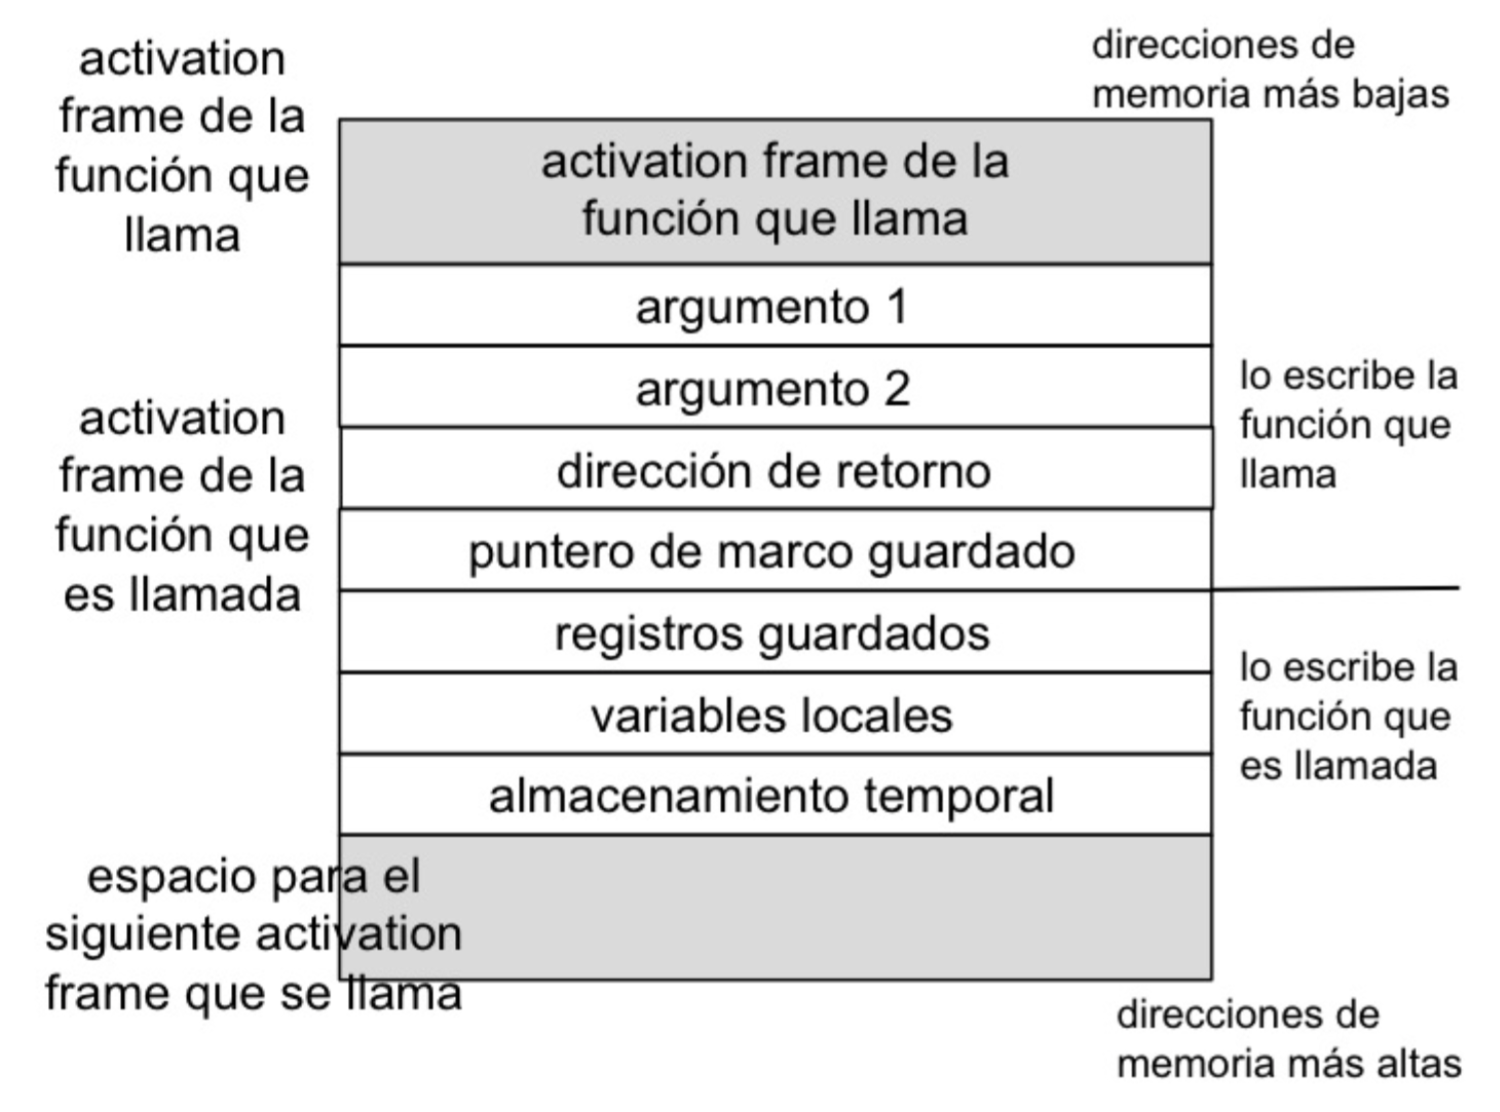
\includegraphics[width=8cm, height=6cm]{memoria.png}
\end{center}

\subsubsection{Ejemplo de activation record}

\begin{center} 	
		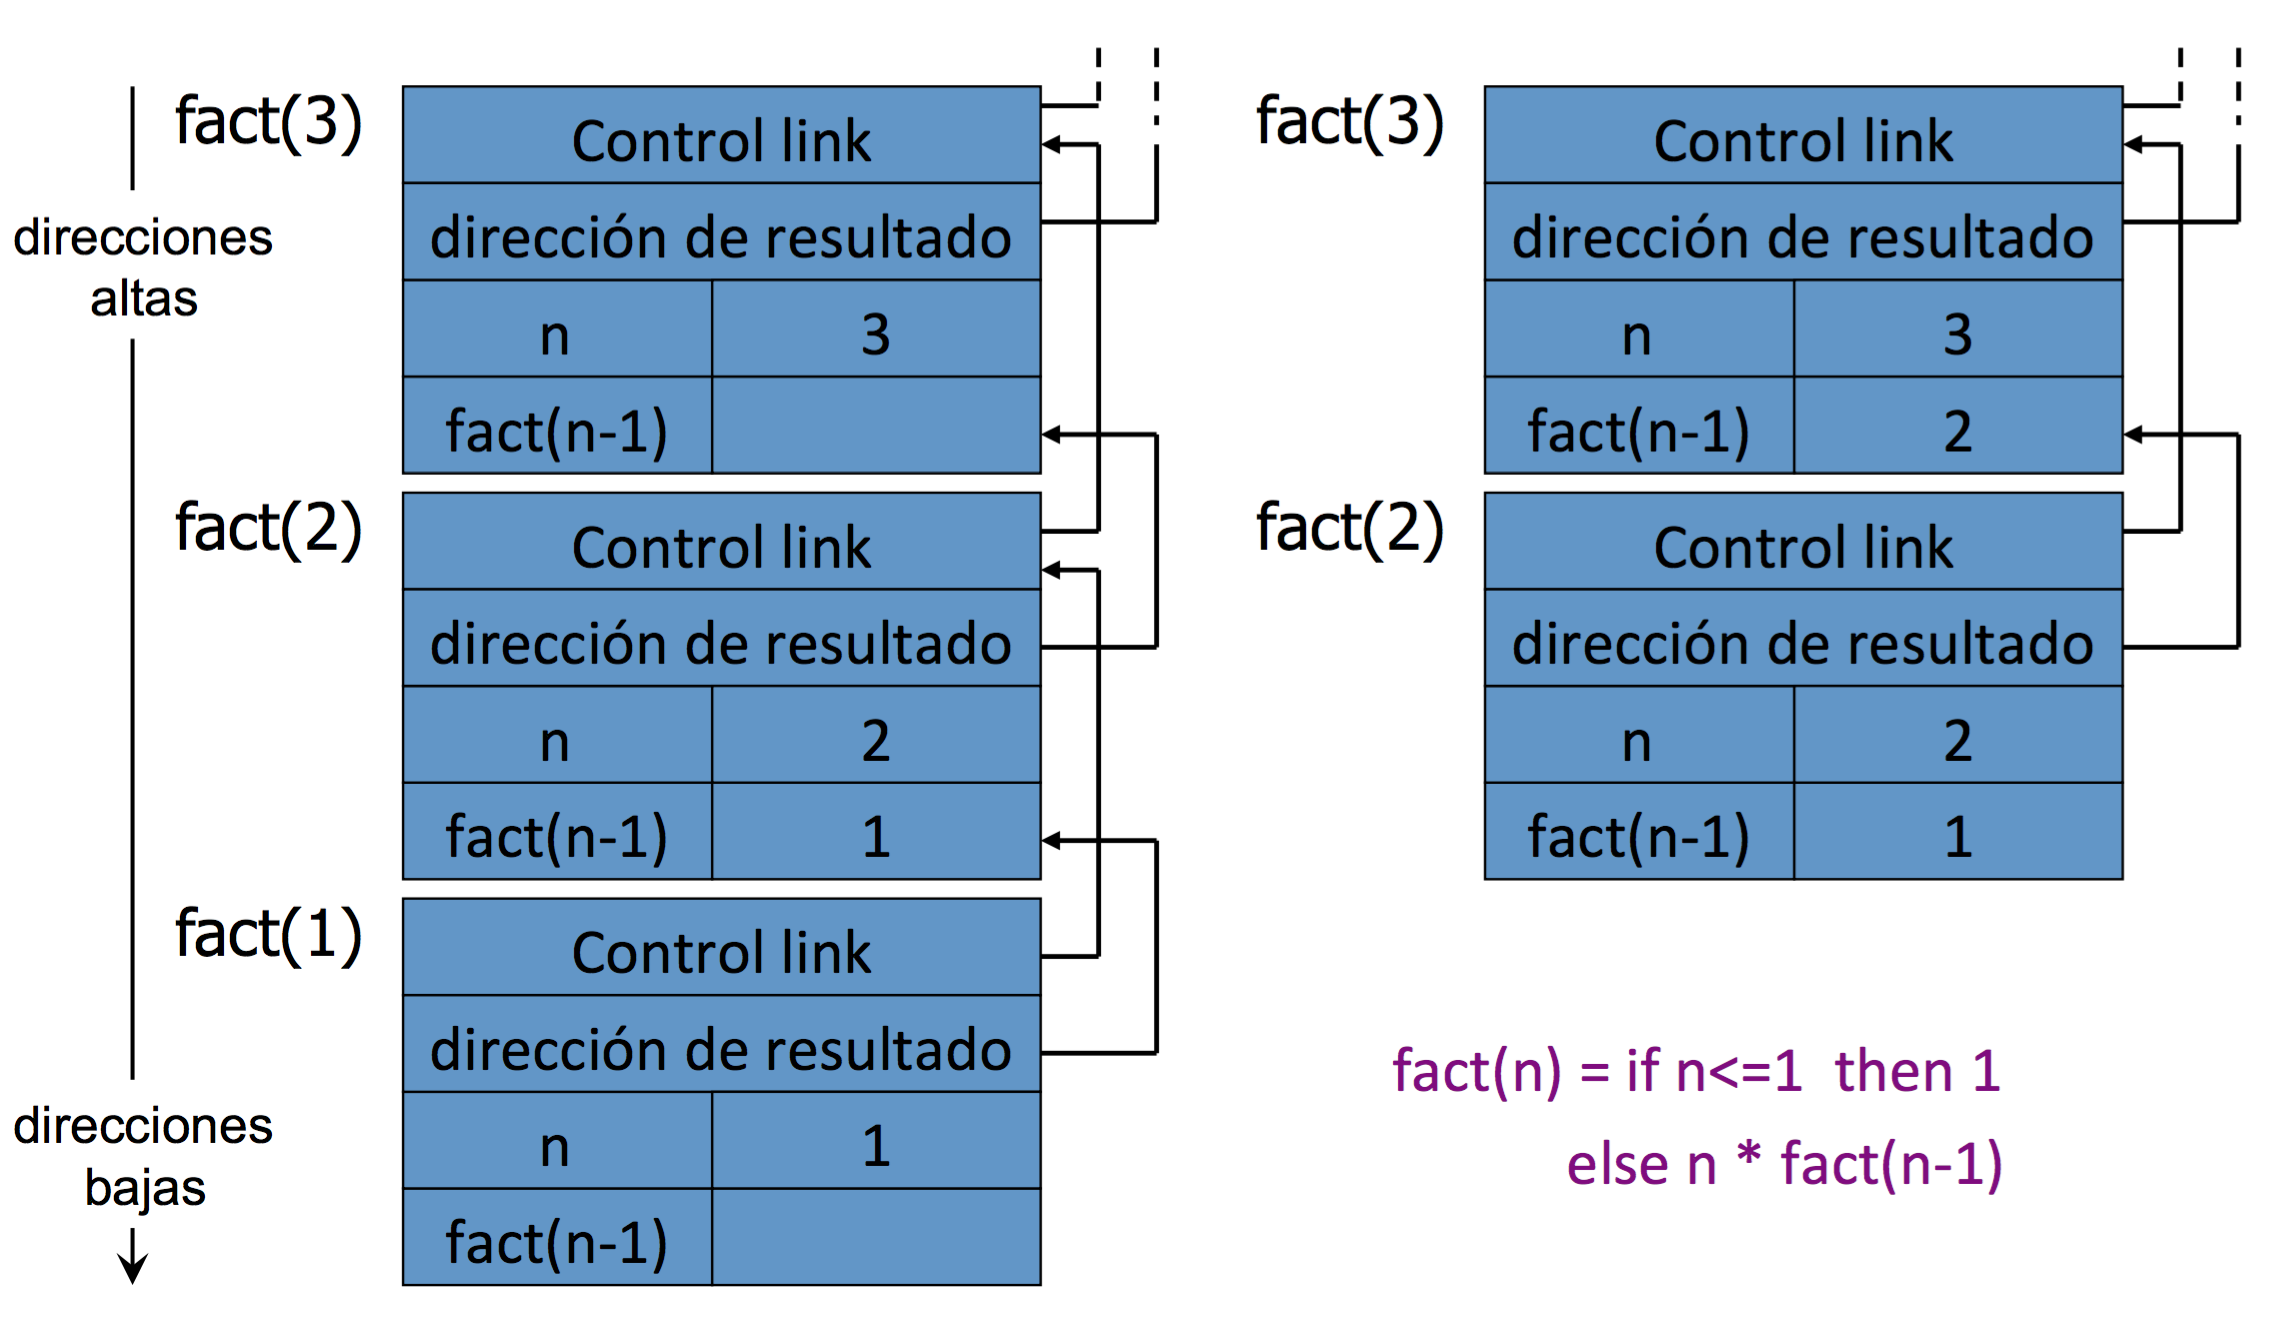
\includegraphics[width=10cm, height=8cm]{factorial.png}
\end{center}


\chapter{Control de la ejecución}

\section{Pasaje de parámetros}
\begin{enumerate}
	\item \underline{Pasaje por valor:} 
	\begin{itemize}
	\item La función que llama pasa el r-valor del argumento a la función. Es 
	necesario computar el valor del argumento en el momento de la llamada. 
	Reduce el \textit{aliasing} (dos identificadores para una sola ubicación en 
	memoria)
	\item  La función no puede cambiar el valor de la variable de la función 
	que llama
	\item Ejemplos: C, Java, Scheme. Se pueden pasar punteros si queremos 
	que se pueda modificar el valor de la variable de la función que llama
	\end{itemize}

	\item \underline{Pasaje por referencia:}
	\begin{itemize}
	\item La función que llama pasa el l-valor del argumento a la función. Se 
	asigna la dirección de memoria del argumento al parámetro. Aumenta el 
	\textit{aliasing}
	\item La función puede modificar la variable de la función que llama
	\item Ejemplos: C++, PHP
	\end{itemize}

	\item \underline{Pasaje por valor-resultado:}
	\begin{itemize}
	\item Intenta tener los beneficios de llamada por referencia (efectos 
	secundarios en los argumentos) sin los problemas de \textit{aliasing}
	\item Hace una copia en los argumentos al principio, copia las variables 
	locales a los argumentos actuales al final del procedimiento. Asi los 
	argumentos son modificados.
	\item Se comporta como llamada por referencia sin la presencia de 	
	\textit{aliasing}
	\item Cuidado: el comportamiento depende del orden en que las 
	variables locales se copian.
	\item Ejemplos: BBC BASIC V
	\end{itemize}
	
	\item \underline{Pasaje por nombre:}
	\begin{itemize}
	\item En el cuerpo de la función se sustituye textualmente el argumento 
	para cada instancia de su parámetro. Se implementó para Algol 60 pero 
	sus sucesores no lo 	incorporaron
  	\item Es un ejemplo de ligado tardío. La evaluación del argumento se 
  	posterga hasta que efectivamente se ejecuta en el cuerpo de la función.
	Asociado a evaluación perezosa en lenguajes funcionales (ej: Haskell)
	\end{itemize}
	
	\item \underline{Pasaje por necesidad:}
	\begin{itemize}
	\item Variación de call-by-name donde se guarda la evaluación del 
	parámetro después del primer uso
	\item Idéntico resultado a call-by-name (y más eficiente) si no hay 
	efectos secundarios
	\item El mismo concepto que lazy evaluation
	\end{itemize}

\end{enumerate}

\begin{center} 	
		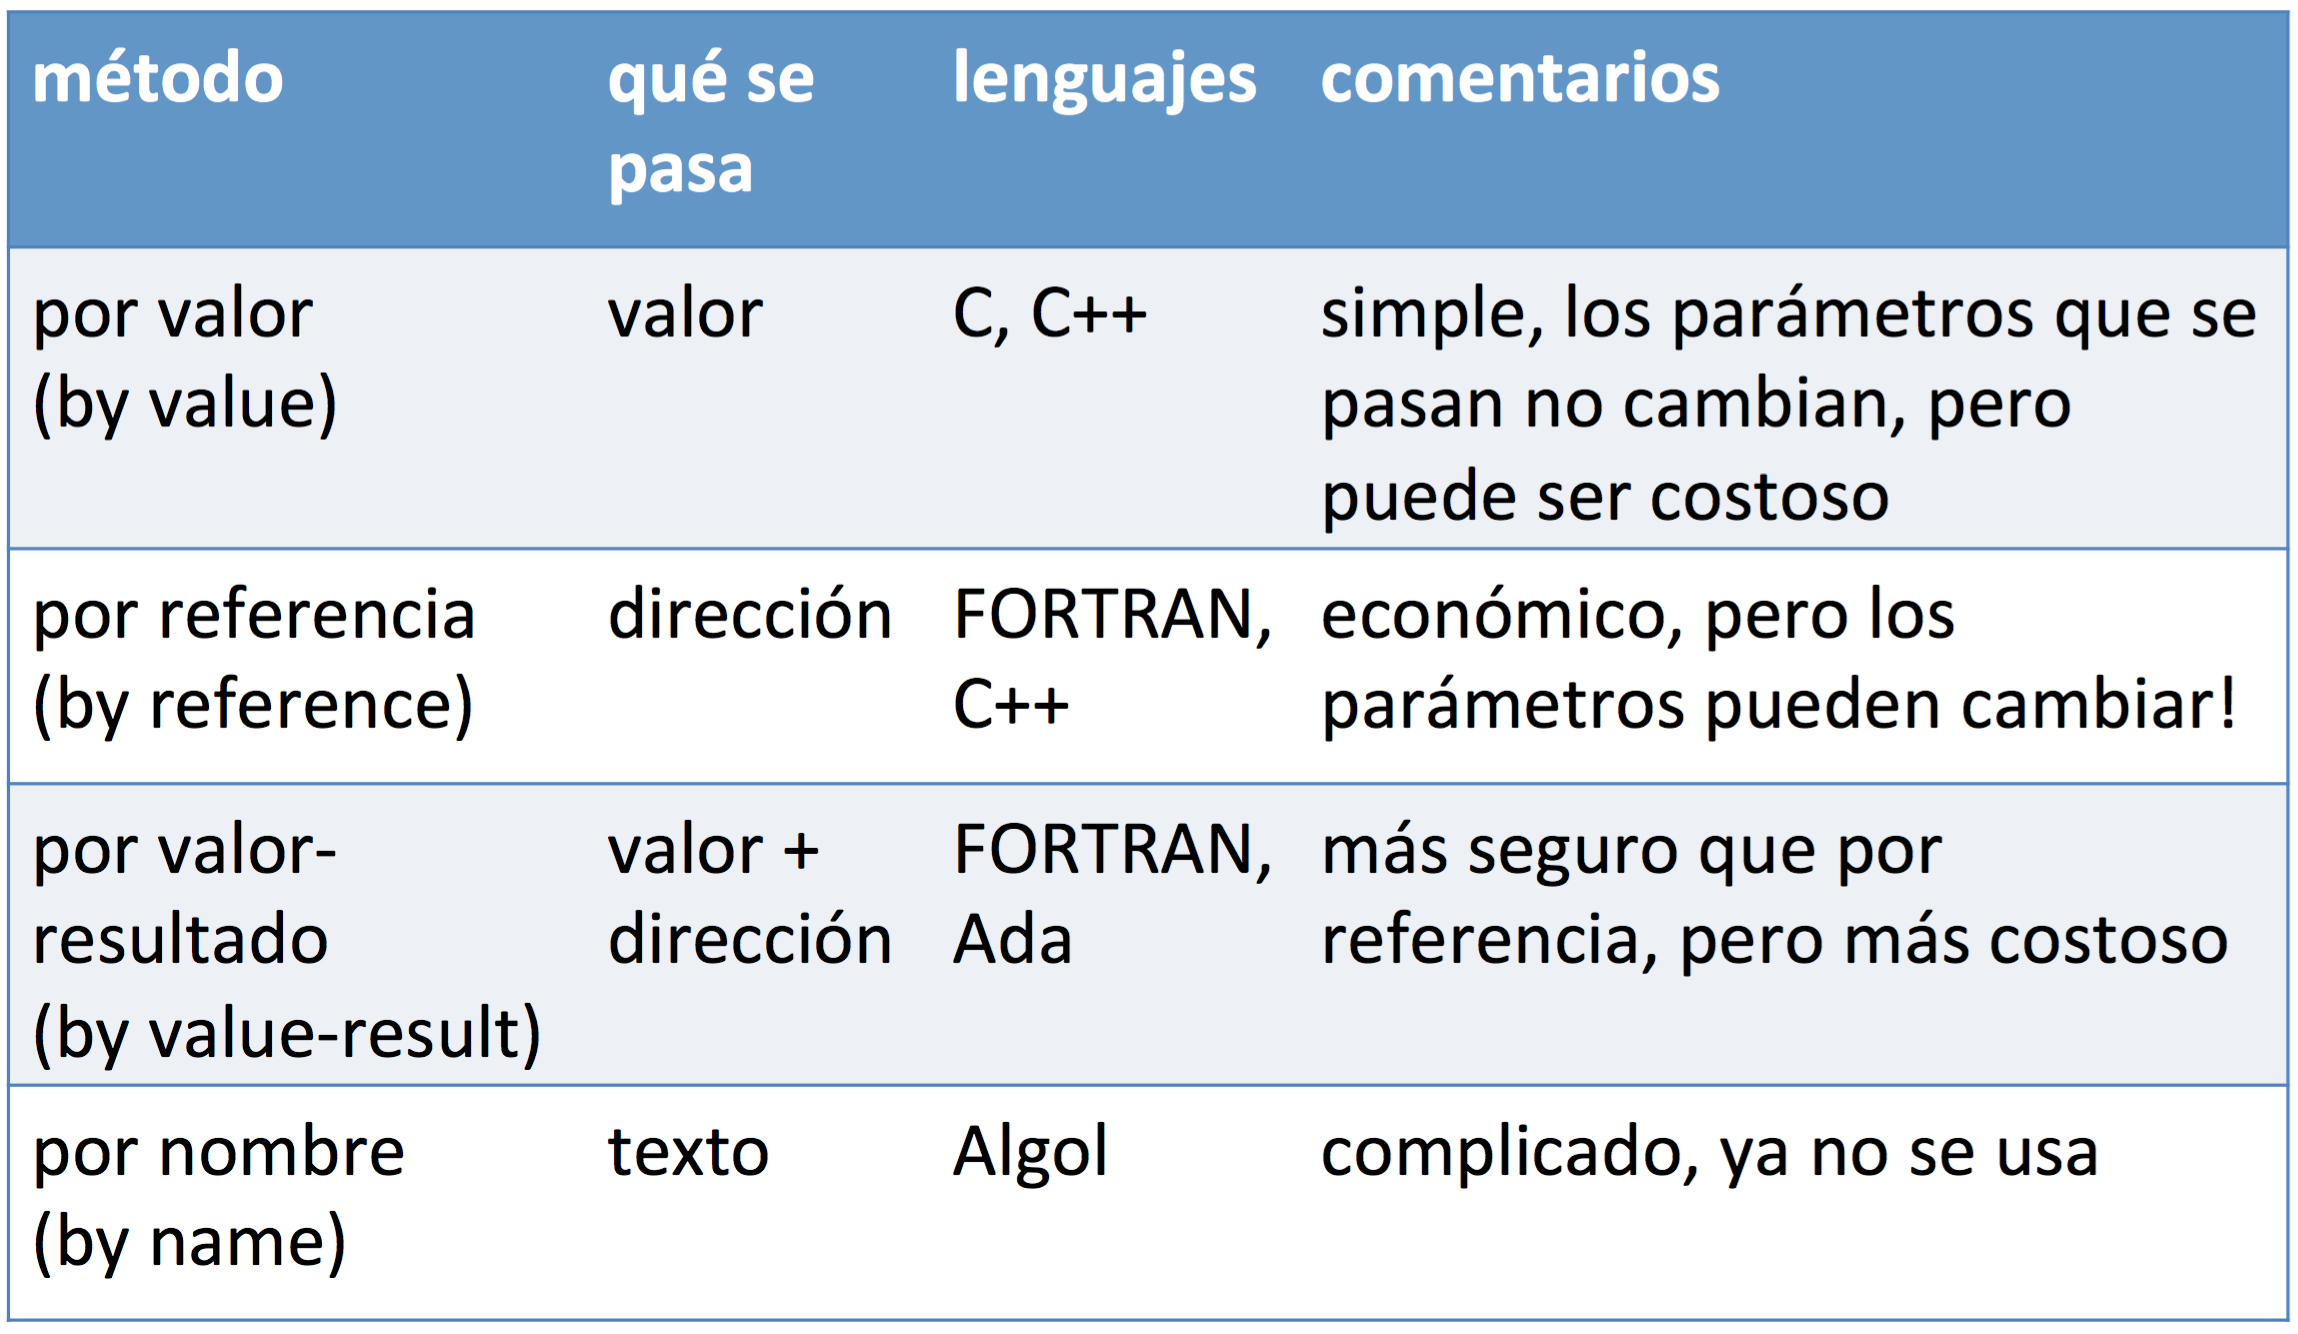
\includegraphics[width=12cm, height=8cm]{resumenpasajes.png}
\end{center}

\section{Alcance}
\par Si un identificador \verb|x| aparece en el cuerpo de una función, pero
\verb|x| no se declara dentro de la función, entonces el valor de
\verb|x| depende de alguna declaración fuera de la función. En esta
situación, la ubicación de \verb|x| está fuera del registro de
activación para la función y es una variable global a esa
función. Debido a que \verb|x| ha sido declarada en otro bloque, el
acceso a una \verb|x| libre o global consiste en encontrar el registro
de activación pertinente en la pila.

Hay dos políticas principales para buscar la declaración adecuada de
un identificador global:

\begin{description}
\item \underline{Alcance estatico:} un identificador global se refiere al identificador con ese nombre que se declara en el bloque contenedor más cercano del texto del programa.
\item \underline{Alcance dinamico:} un identificador global se refiere al identificador asociado con el registro de activación más reciente.
\end{description}

\par Aunque la mayoría de los lenguajes actuales de programación de
propósito general utilizan alcance estático para las declaraciones de
variables y funciones, el alcance dinámico es un concepto importante
que se utiliza en lenguajes de propósito específico y en
construcciones especializadas como las excepciones. Algunos lenguajes
con alcance dinámico son los dialectos antiguos de Lisp, los lenguajes
de marcado Tex/LaTex, las excepciones y las macros.

\begin{center} 	
		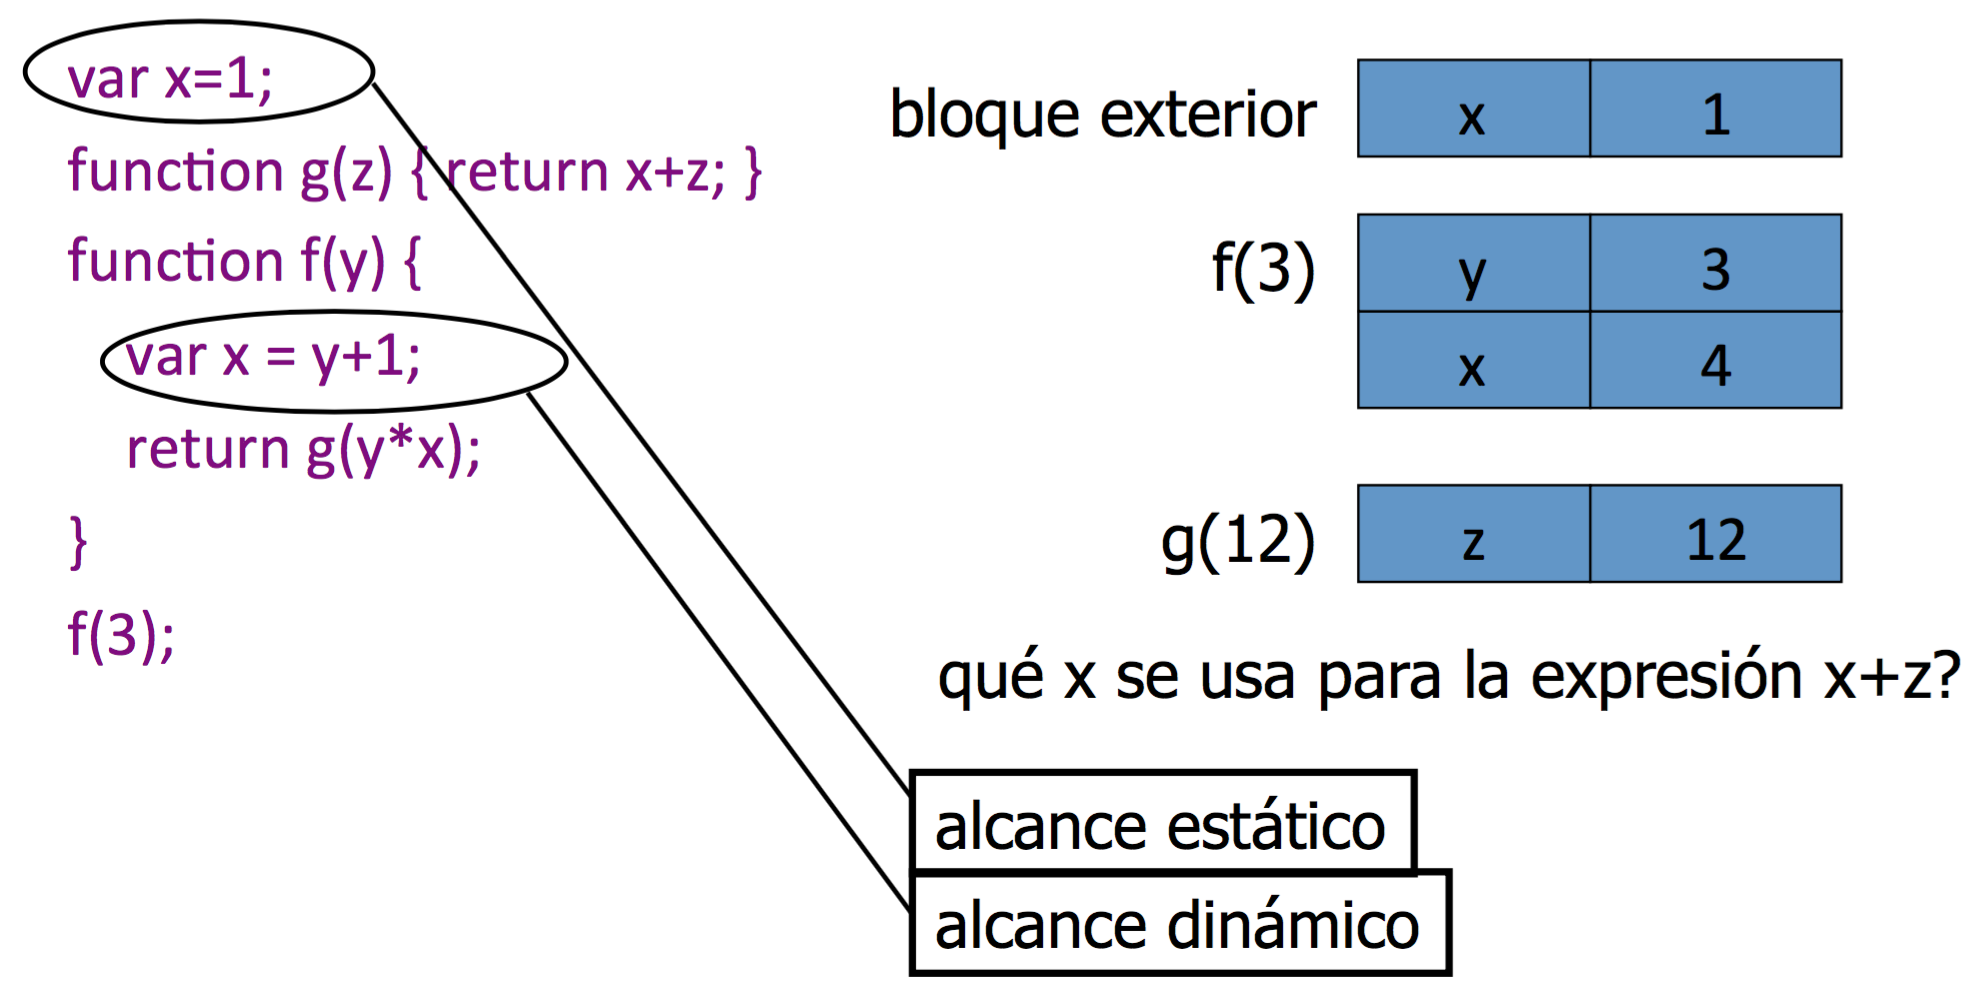
\includegraphics[width=12cm, height=6cm]{estaticodinamico.png}
\end{center}

\section{Alto orden}

\subsection{Funciones de primera clase}
Un lenguaje tiene funciones de primera clase si las funciones pueden ser declaradas 
dentro de cualquier alcance,
pasadas como argumentos a otras funciones y,
devueltas como resultado de funciones.
En un lenguaje con funciones de primera clase y con alcance estático, un valor de 
función se representa generalmente por una clausura, un par formado por un 
puntero al código del cuerpo de una función y otro puntero a un activation record.
Veamos un ejemplo de función en ML que requiere a otra función como argumento:

     1
fun map (f, nil) = nil | map(f, x::xs) = f(x) :: map(f, xs)

La función map toma una función f y una lista m como argumentos y aplica f a cada 
elemento de m en orden. El resultado de map(f, m) es la lista de resultados f(x) para 
elementos x de la lista m. Esta función es útil en muchos programas en los que se 
usan listas. Por ejemplo, si tenemos una lista de tiempos de vencimiento para una 
secuencia de eventos y queremos incrementar cada tiempo de vencimiento, 
podemos hacerlo pasando una función de incremento a map.
\subsection{Pasar funciones a otras funciones}



\section{Recursión a la cola}
\par Una optimización que realizan los compiladores es la llamada eliminación de la recursion a la cola. Para las funciones recursivas a la cola, que describimos a continuación, se puede reutilizar un activation record para una llamada recursiva a la
función. Esto reduce la cantidad de espacio de la pila que usa una
función recursiva, y evita llegar a problemas por límites de hardware
como el llamado {\it stack overflow}, en el que la ejecución de un
programa requiere más espacio del que hay disponible en la pila.
Una llamada a \verb|f| en el cuerpo de \verb|g| es una
llamada de la cola si \verb|g| devuelve el resultado de la llamada
\verb|f| sin ningún cálculo adicional. Una función \verb|f| es recursiva de cola si todas las llamadas recursivas en el cuerpo de \verb|f| son llamadas a la cola a \verb|f|. 

Veamos como ejemplo la función recursiva a la cola que calcula el factorial:

\begin{tabbing}
fun factcola(n,a) = if n <= 1 then a else factcola(n-1, n * a);
\end{tabbing}



\begin{center} 	
		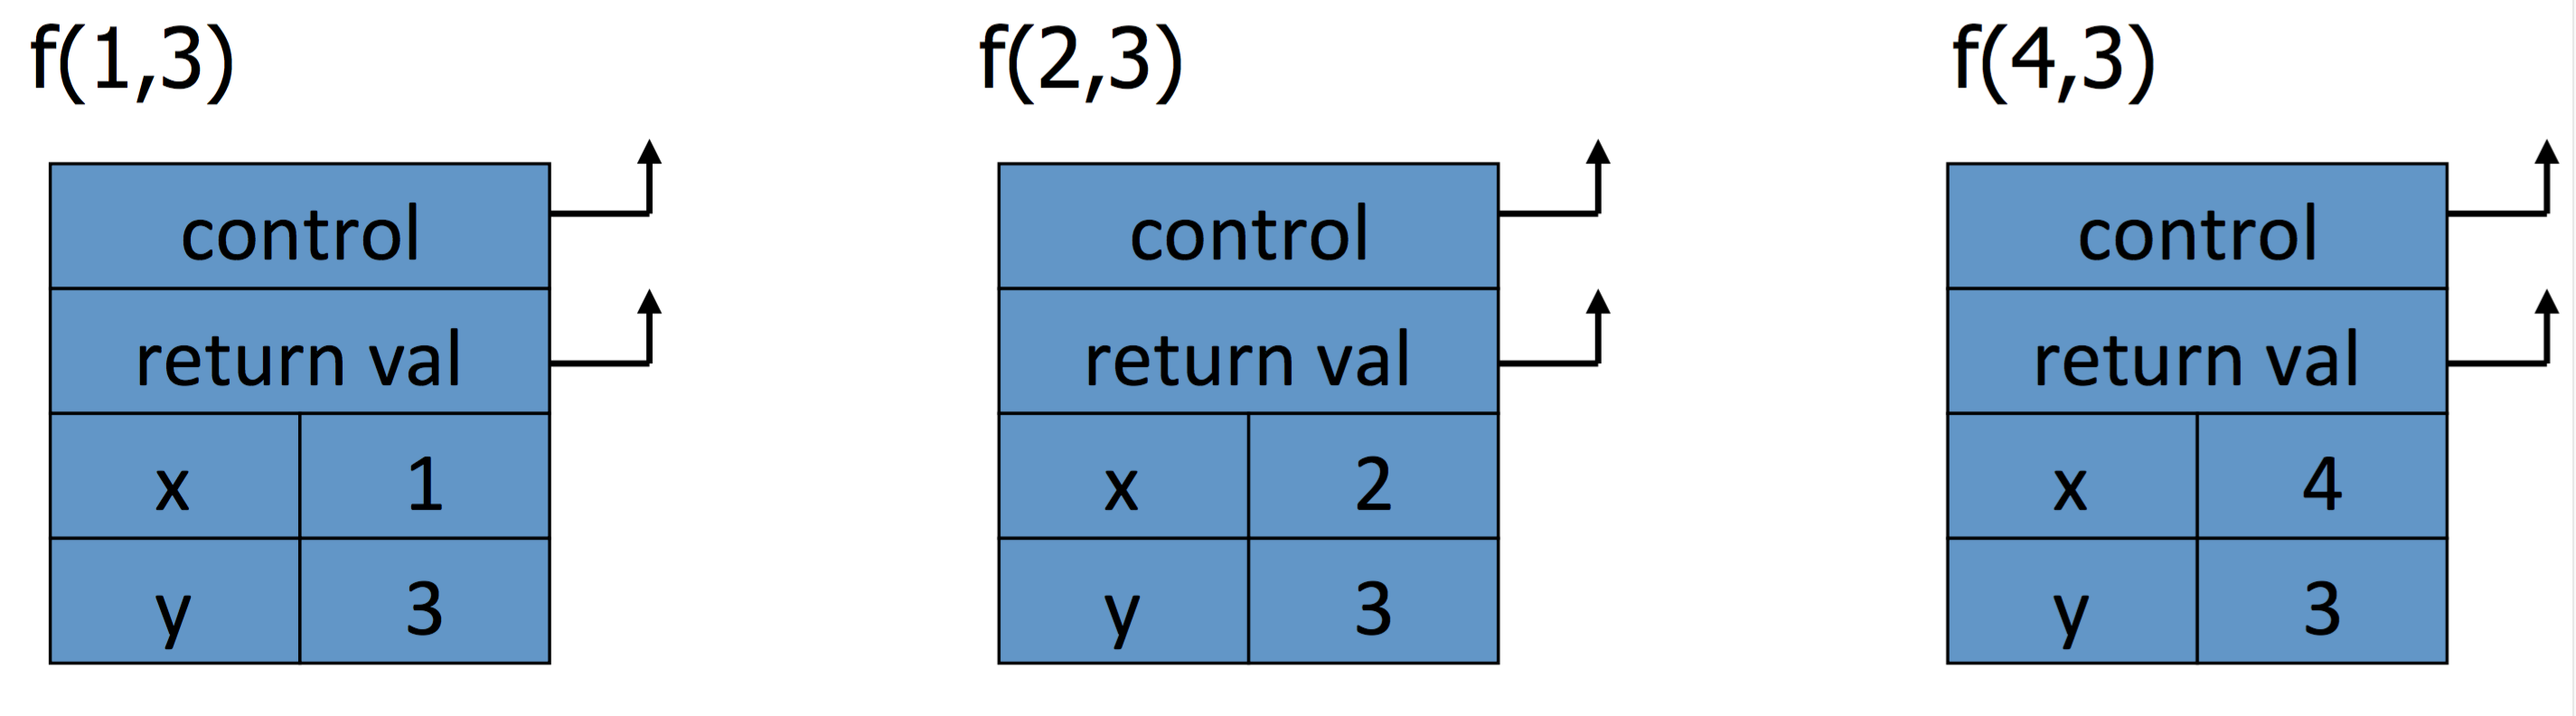
\includegraphics[width=12cm, height=6cm]{factorial2.png}
\end{center}


\section{Excepciones}


\chapter{Orientación a objetos}




\end{document}
